\section{LCD-Bibliothek}
\subsection{Aufgabenstellung}
Schreiben Sie eine Bibliothek zur Ansteuerung des LC-Displays auf dem EDAdsPIC33-Board:
\begin{itemize}
	\item Initialisierung (blocking Code erlaubt)
	\item Zyklisches Kopieren eines Schattenspeichers in den Display-Speicher\newline
			(non-blocking code).
\end{itemize}

\subsubsection*{Hinweise zur Implementierung}

Literatur:
\begin{itemize}
	\item DiJasio(2012): Chapter 9\newline
			\url{https://www.dropbox.com/sh/4bwfkqux88a3j62/AAAhId8mi25vsYaToLJbrS1Ba?dl=0\&preview=09_Glass_Bliss.pdf}
	\item Datenblatt FDCC1602L-NSWBBW-91LE, \newline \url{http://farnell.com/datasheets/653662.pdf}
	\item Datenblatt Displaycontroller \newline
			\url{https://sparkfun.com/datasheets/LCD/HD44780.pdf}\newline
			\url{http://download.maritex.com.pl/pdfs/op/TC1602E-06H.pdf}
	\item Simulator \newline
	 \url{http://dinceraydin.com/djlcdsim/djlcdsim.html}
	
\end{itemize}

Vorgehensweise:
\begin{itemize}
	\item Schreiben Sie zunächst eine Funktion putLCD(), die ein Zeichen auf dem Display ausgibt (blocking code)
	\item Ändern Sie die Funktion so, dass sie kooperativ wird.
	\item Implementieren Sie anschließend das Kopieren des Schattenspeichers
\end{itemize}


\subsection{Lösung}
Die Initialisierung des LCD-Controllers wurde wie im Datenblatt beschrieben umgesetzt. Die im Datenblatt vorgeschlagene Initialisierungssequenz ist in Abbildung \ref{image:lcdinit} (Seite \pageref{image:lcdinit}) abgebildet. Die Funktion \texttt{initMyLCD()} ist in Listening \ref{lst:lcdinit} (Seite \pageref{lst:lcdinit}) zu finden.\newline
\newline
Alle Funktionenprototypen der edaPIC33LCD-Library sind in Listening \ref{lst:lcdlib} (Seite \pageref{lst:lcdlib}) zu finden.\newline
Eine Ausführliche Beschreibung und alternativer Quellcode ist in Programming 16-Bit PIC Microcontrollers in C (Di Jasio) - Chapter 9 zu finden.\newline

\subsubsection*{Abstrahierte Verwendung des LCD}
Um die Verwendung des LCD zu vereinfachen wurde eine Funktionalität entwickelt, welche einen Schattenspeicher zyklisch auf das LCD schreibt. Hierfür wurden die Funktionen in Listing \ref{lst:writedatatolcd} realisiert.\newline

%Shadow String Prototypen
\begin{lstlisting}[frame=htrbl, caption={Funktionsprototypen für Schattenspeicher Funktionalität}, label={lst:writedatatolcd}]
extern char ShadowString[32]; 
void setLCDLine(const char* pStr, uint8_t ui8Line);
void sendDataToLCD();
\end{lstlisting}
Der Funktion \texttt{setLCDLine(pStr, Line)} wird ein String und die gewünschte Zeile des LCD übergeben. Der übergeben String (max. 16 Zeichen) wird in den \texttt{ShadowString} kopiert. Je nach übergebener Zeile werden die Daten ab \texttt{ShadowString[0]} (Zeile 0) bzw ab \texttt{ShadowString[16]} (Zeile 1) gespeichert.\newline
Ist der übergebene String (\texttt{pStr}) kleiner als 16 Zeichen, so wird die restliche Zeile von \texttt{ShadowString} mit Leerzeichen gefüllt (dies vereinfacht die Programmierung der Funktion \texttt{sendDataToLCD()} ). Ist der übergebene String größer als 16 Zeichen, so werden nur die ersten 16 Zeichen kopiert. \newline
Der String \texttt{pStr} muss zwingend nullterminiert sein (Ende gekennzeichnet durch \texttt{'$\ensuremath{\backslash}0$'}). \newline
Die Funktion \texttt{sendDataToLCD()} ist so programmiert, dass bei einem Funktionsaufruf zuerst das Busy-Flag des LCD abgefragt. Anschließend wird, wenn der LCD nicht beschäftigt ist, ein Zeichen des \texttt{ShadowString} an den LCD gesendet. Im nächsten Funktionsaufruf wird dann das nächste Zeichen an den LCD gesendet, oder (wenn nötig) den LCD Cursor auf Zeile 2 setzen, bzw. auf Zeile 1.\newline
\newline
In Abbildung \ref{image:LCD_busy_flag} ist das Busy-Flag des LCD abgebildet. Das LCD benötigt zum schreiben eines Characters ca 30us.
\begin{figure}[!h]
	\centering
	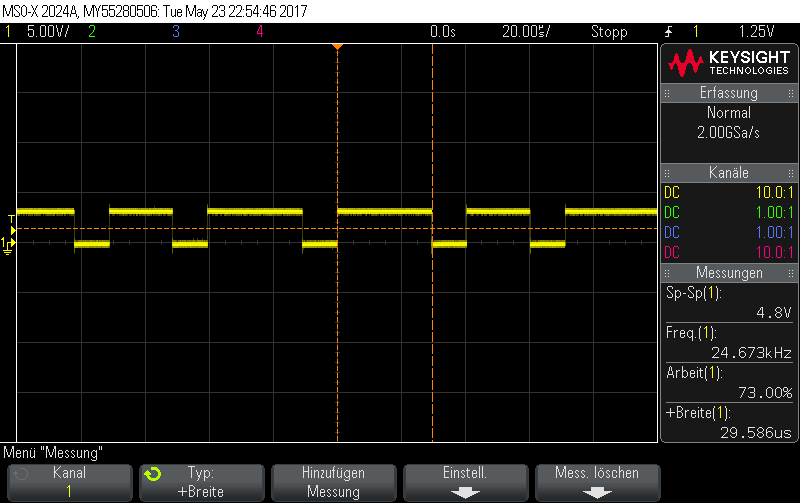
\includegraphics[width=0.65\textwidth]{Images/LCD_busy_flag}
	\caption[NonBlockingCode]{Busy-Flag des LCD Display}
	\label{image:LCD_busy_flag}
\end{figure}

